\chapter{Kvalitetsarbete i praktiken}
\label{cha:indiv-report-wallstrom}
\chapterprecis{\LARGE{---- Fredrik Wallström ----}}


\section{Inledning}
\label{sec:introduction-wallstrom}

De flesta företag ute på marknaden idag strävat mot att utveckla bättre produkter och tjänster. Detta leder till att kvalitetsarbetet i utvecklingen av dessa produkter och tjänster spelar en alltmer betydande roll. Kvalitetsarbetet är ett problem att effektivisera för att hinna med dagens utveckling och är generellt ett komplext ämne att behandla. Det står dock klart att det är en viktig komponent i utveckling av bättre produkter och tjänster.

\subsection{Syfte}
\label{sec:purpose-wallstrom}

Syftet med denna rapport är att ta reda på vad det innebär att kvalitetssäkra ett mjukvarusystem och vilka metoder det finns för ändamålet. Syftet är också att se över hur kvalitetsarbetet används i praktiken, samt om det finns möjligheter att utveckla och effektivisera detta arbete. Detta undersöks eftersom det blir alltmer aktuellt på grund av den snabba utvecklingen av produkter och tjänster.

\subsection{Frågeställning}
\label{sec:issue-wallstrom}

De frågeställningar som denna rapport kommer ta upp är:

\begin{enumerate}
	\item Vad är effekterna av att kvalitetssäkra mjukvaran för en produkt med den specifika metoden kodgranskning?
	\item Vad är de egentliga kostnaderna med att kvalitetssäkra en produkts mjukvara med kodgranskning, kommer effekterna för kvalitetssäkringen kompensera för den faktiska tidsåtgången?
\end{enumerate}

\subsection{Avgränsningar}
Denna rapport kommer endast att undersöka vad den specifika metoden kodgranskning har för påverkan på kvaliteten hos ett mjukvarusystem. Det finns flera metoder för detta ändamål men dessa kommer alltså inte att undersökas i denna rapport eftersom just kodgranskning har använts under det relaterade kandidatprojektet. En annan avgränsning är att den enkät som genomfördes under experimentet endast skickades ut till 30 personer.

\section{Bakgrund}
\label{sec:background-wallstrom}

Kodgranskning är en vanlig process för att öka kvaliteten på koden och för att utsända kunskap inom projektet där koden är aktiv. Den här studien har genomförts för att se vilken påverkan en modern kodgranskningsprocess har på kvaliteten hos ett mjukvarusystem. 

Studien har också undersökt vad det är som gör att kodgranskning har blivit en viktig del för att kvalitetssäkra ett mjukvarusystem och vad de praktiska fördelarna är med en modern kodgranskningsprocess. Det är alltså intressant att se vilka problem som löses med hjälp av denna process. 

\section{Teori}
\label{sec:theory-wallstrom}
Nedan följer information om de ämnen som behandlas i rapporten. Informationen beskriver vad kvalitetssäkring innebär, vad kodgranskning är för något och hur det specifika kodgranskningsverktyget Gerrit fungerar.

\subsection{Kvalitetssäkring}
Att genomföra en kvalitetssäkrande process innebär enligt definition att "tillhandahålla en försäkran om att programvaruprodukten och processer i produktens livscykel överensstämmer med deras specifika krav och håller fast vid de uppsatta planerna". 
Kvalitetssäkran är en process som genomförs under hela utvecklingen av ett system och inte någonting som går att applicera på ett redan färdigt system \cite{feldman2005quality}.

Det finns flera aktiviteter som kan ingå i en kvalitetssäkrande process, beroende på projekt samt dess kvalitetsmål. Processen kan alltså bestämmas utifrån projektets syfte och mål. En viktig aktivitet i de flesta kvalitssprocesserna är testning, att kontinuerligt testa en produkt leder till att buggar kan hittas och åtgärdas. En annan ofta vanlig aktivitet i en kvalitetssäkrande process är kodgranskning \cite{feldman2005quality}.

\subsection{Kodgranskning}
Kodgranskningsprocessen definierades av Fagan \cite{fagan1999design} och innebär att: "Granskarna som granskar en kods ändringar ska metodiskt följa checklistor för att sedan medverka i gruppmöten tillsammans med kodens författare och diskutera de förslagna ändringarna". En kodgrankningsprocess syfte är att upptäcka fel och fixa dessa fel innan koden integreras med kodbasen \cite{mcintosh2014impact}. 

Fagans \cite{fagan1999design} kodgranskningsprocess har under åren moderniserats till en så kallas modern kodgranskningsprocess. Den moderna kodgranskningsprocessen behåller Fagans ursprungliga metod för processen med skillnaden att checklistorna och gruppmötena istället har utvecklats till att ske online. Detta har antagligen blivit följden eftersom att även samhället har moderniserats till att bli mer beroende av internet \cite{shimagaki2016study}.

Att utföra en kodgranskningsprocess idag är enkelt. Det finns idag verktyg som underlättar en kodgranskningsprocess, till exempel Gerrit. Kodgranskning har dessutom integrerats i olika versionshanteringsverktyg, till exempel GitHub. För att sammanfatta en kodgranskningsprocess så innebär det att en utvecklare föreslår en kodändring, denna kod integreras sedan med kodbasen om den godkänns av de utnämnda granskarna \cite{shimagaki2016study}.


\subsection{Gerrit}
Gerrit är ett av de moderna kodgranskningsverktyg som finns idag. Gerrit är inte en process utan är till för att underlätta en kodgranskningsprocess. Att använda Gerrit i ett projekt fungerar som en vanlig modern kodgranskningsprocess. Det som Gerrit underlättar med är det grafiska gränssnittet, det hjälper till att få en enkel och snabb överblick över statusen i processen \cite{mcintosh2014impact}.

\section{Metod}
\label{sec:method-wallstrom}

För att förstå effekterna av att genomföra en kodgranskningsprocess samt att inse vad de egentliga kostnaderna är med att kvalitetssäkra en produkt har en litteraturstudie genomförts. Litteraturstudien bestod av att analysera och bearbeta olika vetenskapliga rapporter som var relevanta för ämnet ifråga. De utvalda rapporterna hade genomfört intressanta experiment och utredningar som kändes trovärdiga.

För att undersöka dessa frågor med en koppling till praktiken så har även ett praktiskt experiment gjorts på studenter ifrån Linköpings universitet. Dessa studenter har genomfört ett projekt där fokus var att leverera ett färdigt system med hög kvalitet till kund. Experimentet bestod av att studenterna skulle svara på en enkät om hur det är att jobba med en kvalitetssäkrande process. Frågorna som studenterna fick svara på var följande:

\begin{itemize}
	\item Hur anser du det är att jobba med en kvalitetssäkrande process, är det positivt eller negativt, om man tar den faktiska tidsåtgången i åtanke?
	\item Har du jobbat med den specifika metoden kodgranskning för att säkerställa kvaliteten på en produkt?
	\item Tycker du att kodgranskning hjälper att kvalitetssäkra en produkt?
	\item Anser du graden av deltagande människor i kodgranskningen hjälper eller försämrar kvaliteten hos produkten? Blir det för komplicerat att anordna möten, tidsåtgången blir för stor, det tar för lång tid att få koden godkänd med mera.
	\item Har du några övriga tankar om att arbeta med en kvalitetssäkrande process eller med kodgranskning?
\end{itemize}

Detta experiment valdes eftersom att enbart utgå ifrån litteraturstudier inte ger en representativ bild av de relevanta kvalitetsfrågorna. Experimentets syfte var att se hur kvalitets\-arbete fungerar i praktiken. Det är också intressant att se hur detta experiment skiljer sig ifrån resultatet av litteraturstudien. Det valdes studenter från Linköpings universitet eftersom det var viktigt att studenterna har jobbat med en kvalitetssäkrande process, vilket de har gjort under deras kandidatarbete.

\section{Resultat}
\label{sec:results-wallstrom}
Nedan följer resultatet ifrån den litteraturstudie som genomförts och ifrån den enkät som genomfördes på studenter ifrån Linköpings universitet. 

\subsection{Litteraturstudie}
McIntosh et al. \cite{mcintosh2014impact} visar med en empirisk studie vilken påverkan en modern kodgranskningsprocess har på kvaliteten hos ett mjukvarusystem. McIntosh analyserar huruvida det finns en relation mellan kodgranskning och kvalitet genom att studera 3 stycken projekt. Dessa projekt drivs av en kodgranskningsprocess som använder sig av verktyget Gerrit. Studierna går ut på att undersöka hur kvaliteten påverkas beroende på hur stor del av koden som har blivit kodgranskad och hur många recensenter som deltagit i kodgranskningen. Det visar sig att både andelen kod granskad och hur många som har deltagit i kodgranskningen har en koppling till kvalitet. Låg andel kod granskad samt lågt deltagande visar sig skapa mellan 2-5 stycken extra defekter efter produktlansering. McIntosh bekräftar med sin empiriska studie att dåligt granskad kod har negativa effekter på kvaliteten hos ett mjukvarusystem.

Beller et al. \cite{beller2014modern} visar med en empirisk studie vad de praktiska fördelarna är med en modern kodgranskningsprocess. Studien går ut på att manuellt klassificera 1400 ändringar som gjorts i en kodgranskningsprocess för öppen källkod. Beller kommer fram till att 7-35 \% av de granskade kommentarerna kasseras samt att 10-22 \% av ändringarna inte utlöstes av en kommentar ifrån kodgranskningen. Bellers slutsats är att en homogen kodgranskning, det vill säga en likartad kodgranskning beroende på vem som utför den, leder till samma antal ändringar i koden oberoende på granskaren.

\subsection{Enkät}
De sammanfattade resultaten ifrån den genomförda enkäten presenteras nedan, för mer detaljerade resultat, se bilaga \ref{appendix:svar_enkat_kvalitet}.
\begin{itemize}
	\item \textbf{100\%} anser att det är positivt att jobba med en kvalitetsäkrande process.
	\item \textbf{88\%} har jobbat med den specifika metoden kodgranskningen för att säkerställa kvaliteten hos en produkt.
	\item \textbf{100\%} anser att kodgranskning hjälper till att kvalitetssäkra en produkt.
\end{itemize}
Figur \ref{fig:grade_participation} nedan visar resultatet från frågan om graden av deltagande människor i en kodgranskningsprocess hjälper eller försämrar kvaliteten hos en produkt.

\begin{figure}[H]
	\centering
	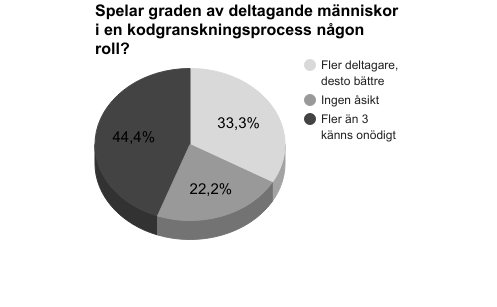
\includegraphics[width=100mm]{figures/grade_participation.png}
	\caption{Visar resultatet från om graden av deltagande människor i en kodgranskningsprocess spelar någon roll.}
	\label{fig:grade_participation}
\end{figure}

\section{Diskussion}
\label{sec:discussion-wallstrom}
Resultatet av den genomförda enkäten visar att effekterna av en kodgranskningsprocess är positiva. 100 \% anser att kodgranskning hjälper till att kvalitetssäkra en produkt. Det är endast få personer som inte använt sig av den specifika metoden kodgranskning för att kvalitetssäkra en produkt, utan istället använt sig av parprogrammering. Denna data är inte tillräcklig och är en avgränsning i denna studie, för en mer representativ bild skulle det krävas större mängd data. 

Det intressanta med resultatet ifrån enkäten är att 44,4 \% av de som deltog anser att om fler än tre personer deltar i en kodgranskningsprocess finns det risk att tidsåtgången inte kompenserar för den faktiska vinsten med granskningen. Detta är också något som Beller et al. \cite{beller2014modern} kommer fram till i sin studie angående vilka problem som löses med hjälp av kodgranskning. Beller anser att en homogen kodgranskning, det vill säga en likartad kodgranskning beroende på vem som utför den, leder till samma antalet ändringar i koden oberoende av vem som granskar. Det spelar alltså inte någon roll vem som granskar koden, den kommer heller inte blir bättre desto fler som granskar. Resultatet tyder alltså på att en kodgranskningsprocess inte bör innehålla fler deltagande personer än tre för att kvalitetssäkra produkten. 

Samtidigt visar McIntosh et al. \cite{mcintosh2014impact} att kodgranskningsprocesser med lågt deltagande uppskattningsvis innehåller upp till 5 stycken defekter efter lansering, vilket kan låta som en kontradiktion till Bellers et al. \cite{beller2014modern} resultat. McIntosh specificerar dock inte att det finns ett optimalt antal personer som ska delta i en kodgranskningsprocess för att göra den så effektiv och kvalitetssäkrande som möjligt. Den intressanta fråga som jag då ställer mig är om det finns ett optimalt antal deltagande personer i en kodgranskningsprocess? Det är en fråga som utifrån egna slutsatser inte finns något svar på. Det är en bred fråga och beror på hur stort projektet är och vad det finns för kvalitetsmål på produkten. Desto högre kvalitetsmål, desto fler personer bör delta i kodgranskningsprocesserna känns intuitivt som ett bra tillvägagångssätt. Denna studie visar dock att så inte är fallet, kodgranskningen riskerar att bli ineffektiv vilket således kan leda till en icke komplett produkt. Det här är en intressant frågeställning som kräver vidare efterforskning. Även här finns det såklart avgränsningar som bör tas med i åtanke. Dels innehåller inte enkäten tillräckligt med data och därtill skulle det även behövas göra en mer omfattande litteraturstudie för att få en representativ bild över situationen.

\section{Slutsatser}
\label{sec:conclusions-wallstrom}
Utifrån den genomförda enkäten men framförallt utifrån den gjorda litteraturstudien visar denna rapport att kvalitet och kodgranskning har en stark relation. Att genomföra en kodgranskningsprocess visar sig tydligt ha positiva effekter på produktens kvalitet. För att svara på fråga 1 i avsnitt \ref{sec:issue-wallstrom} så tyder resultatet från denna studie på att effekterna av en kodgranskningsprocess är positiva ur kvalitetssynpunkt. McIntosh et al. \cite{mcintosh2014impact} visar att en dåligt granskad kod ger upphov till 2-5 stycken extra defekter efter produktlansering.

För att svara på fråga 2 i avsnitt \ref{sec:issue-wallstrom} så tyder resultatet från denna studie att kostnaden för en kodgranskningsprocess kompenserar för den faktiska tidsåtgången. Den genomförda enkäten visade att 100 \% av deltagarna anser att kodgranskning hjälper till att kvalitetssäkra en produkt. Enkäten visar också att graden av deltagande människor i kodgranskningen inte behöver överstiga tre stycken, detta kan leda till onödig tidsåtgång. Det här är även något som bekräftas av Bellers et al. \cite{beller2014modern} studie. Slutsatsen av detta är att effekterna av en kodgranskningsprocess kompenserar den faktiska tidsåtgången så länge antalet personer som granskar inte överstiger tre stycken.


%%%%%%%%%%%%%%%%%%%%%%%%%%%%%%%%%%%%%%%%%%%%%%%%%%%%%%%%%%%%%%%%%%%%%%
%%% person-report.tex ends here
